\documentclass{article}
\usepackage{graphicx}
\usepackage{hyperref}

\begin{document}

\title{The HypeDyn 2 Hypertext Fiction Editor\\Tutorial 1: Nodes, Links and Rules}
% \author{Alex Mitchell}
\date{}

\onecolumn
\maketitle

\tableofcontents


\section{Introduction}
In this tutorial, we will build a basic interactive story in the \textit{HypeDyn 2} hypertext fiction editor. HypeDyn is a tool which lets you create ``hypertext'', a form of writing which usually consists of:

\begin{itemize}
  \item \textit{Nodes}, each containing some text, that
  are normally displayed one at a time in a hypertext reader;
  \item \textit{Links} between these nodes, which provide a connection from one node, or more commonly from a fragment of text in one node, to another node. A reader is usually able to ``follow'' a link to its destination node by, for example, clicking on the link; 
  \item \textit{Rules} that can be attached to a fragment of text or to an entire node, which contain a set of conditions, and a set of actions, such as following a link, which are performed if the rule's conditions are satisfied.
\end{itemize}

In this tutorial, we will be creating a simple hypertext \textit{fiction}. Hypertext fiction usually consists of a story told in hypertext. Most well-known examples of hypertext fiction let the reader explore through a set of nodes, encouraging them to discover different paths through the story. These alternate paths sometimes uncover new information which the reader didn't previously know, thereby altering their perception of the story.

Our example, ``Little Red Riding Hood'', involves the reader exploring several paths through a story. The main path tells a simplified version of the traditional folk tale, about a little girl with a red hood who meets a wolf on the way to visit her Grandmother. An additional side path, which can only be accessed once the reader has visited the last node in the main path, reveals some additional background information about Red's hood.


\begin{figure}[ht]
  \centering
  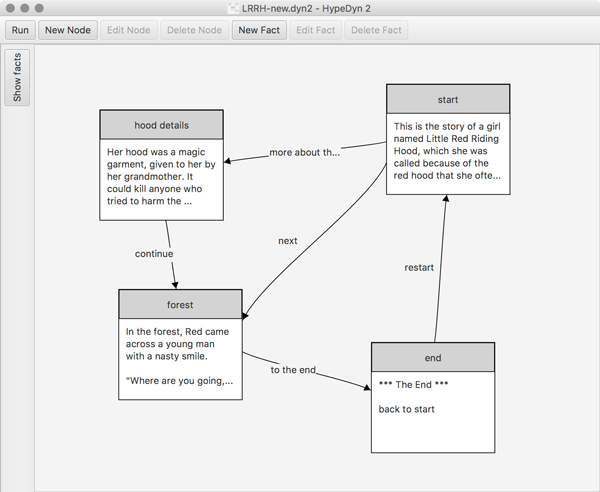
\includegraphics[width=10cm]{images/hypedyn-tutorial-1-figure-1}
  \caption{\textit{The completed ``Little Red Riding Hood'' story.}}
  \label{fig:tut1:completed_story}
\end{figure} 

The nodes and links in the final story are shown in Figure \ref{fig:tut1:completed_story}. Although this is a very simple story, it will involve most of the basic functionality of HypeDyn.

\textit{Note:  HypeDyn is a work-in-progress. If you encounter any errors, please report them as issues on our Github site: \url{https://github.com/narrativeandplay/hypedyn2}.}

\section{Getting started}

First, open HypeDyn by double-clicking on the file \textbf{HypeDyn2.exe} (in Windows) or \textbf{HypeDyn 2.app} (in MacOS). You should see an empty HypeDyn window, as shown in Figure \ref{fig:tut1:hypedyn}.

\begin{figure}[ht]
  \centering
  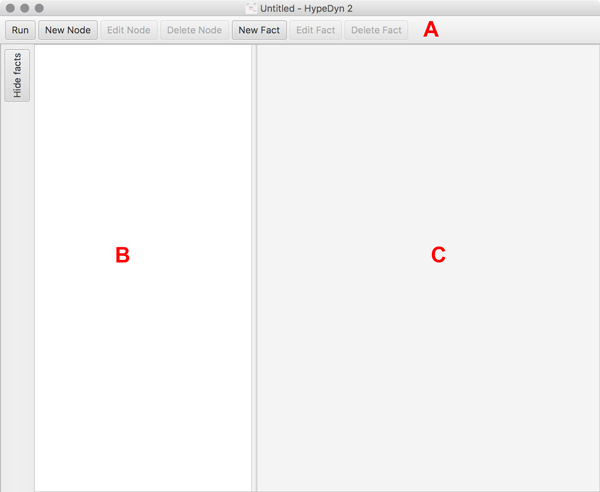
\includegraphics[width=10cm]{images/hypedyn-tutorial-1-figure-2}
  \caption{\textit{The main HypeDyn interface.}}
  \label{fig:tut1:hypedyn}
\end{figure} 

The main HypeDyn interface consists of the \textit{Toolbar} (A), the \textit{Fact list} (B), and the \textit{Map view} (C). The Toolbar contains the functions that we will use to create and edit our nodes. The Fact list contains a list of the \textit{facts} in your story. The Map view displays the nodes and links in your story. The Map view contains two different types of nodes: regular nodes and \textit{anywhere} nodes. We will not be using facts or anywhere nodes in this tutorial. You can hide the Fact list by clicking on the ``Hide facts'' button at the left side of the window.

Before you do anything else, save your file by choosing \textit{Save} from the \textit{File} menu. Make sure that you give the file a \textbf{.dyn2} extension.

\section{Creating a node}

The first thing we need to do is to start creating some nodes. Nodes are the basic building blocks of hypertexts created with HypeDyn.
Each node has: 
\begin{itemize}
  \item A title to identify the node,
  \item Some text content,
  \item A list of text fragments, and
  \item A list of \textit{fragment rules} and \textit{node rules}.
\end{itemize}

We will explain the use of text fragments and rules later in this tutorial. For now, we'll begin by creating the starting node, which represents the first fragment in the story. In this node, we will introduce the main character, Red, and the initial action of the story, the fact that she is walking through the forest.
 
\begin{figure}[ht]
  \centering
  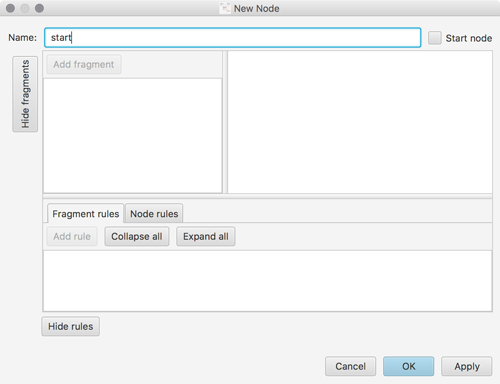
\includegraphics[width=10cm]{images/hypedyn-tutorial-1-figure-3}
  \caption{\textit{Creating a new text node.}}
  \label{fig:tut1:new_node}
\end{figure} 

\begin{enumerate}
  \item To create a new node, click on the \textit{New node} button. A new node will be created in the \textit{New Node} window, as shown in Figure \ref{fig:tut1:new_node}.
  \item Name the new text node ``Start'' by typing in the ``Name'' text field at the top left of the window. 
  \item For now, ignore the rest of this window and just click Ok.
  
  Note: these screenshots are taken on a Mac. The order of the ``Ok'' and ``Cancel'' buttons will be reversed on Windows.
\end{enumerate}
 
Once you've created a node, you should see the node represented in the Map view (see Figure \ref{fig:tut1:first_node}). You can select the
node by clicking on it in the Map view. You can also drag the node around in the Map view by selecting the node and then dragging it. 

\begin{figure}[ht]
  \centering 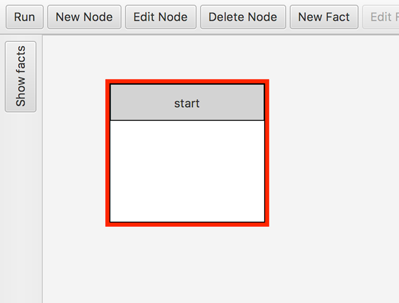
\includegraphics[width=8cm]{images/hypedyn-tutorial-1-figure-4}
  \caption{\textit{Our first node showing in the Map view.}}
  \label{fig:tut1:first_node}
\end{figure} 

Once we have created several nodes and links between them, it can be useful to position them in the Map view so that we can easily see the relationship between them. However, the position of the nodes in the Map view does not change their behaviour in any way. 

You can zoom the Map view using the ``command-plus'' and ``command-minus'' (MacOS) or ``ctrl-plus'' and ``ctrl-minus'' (Windows) keys, and reset the zoom level using ``command-0'' (MacOS) or ``ctrl-0''.

\section{Adding text to a node}

Now that we have our first text node, we need to go in and enter some text.

\begin{enumerate}
  \item Choose the node in the Map view, and then click on the \textit{Edit node} button in the Toolbar. This will open the \textit{Edit Node} window for the node, as shown in Figure \ref{fig:tut1:edit_node}. (Note that you can also open the Edit Node window by double-clicking on the node in the Map view.)
  
\begin{figure}[ht]
  \centering
  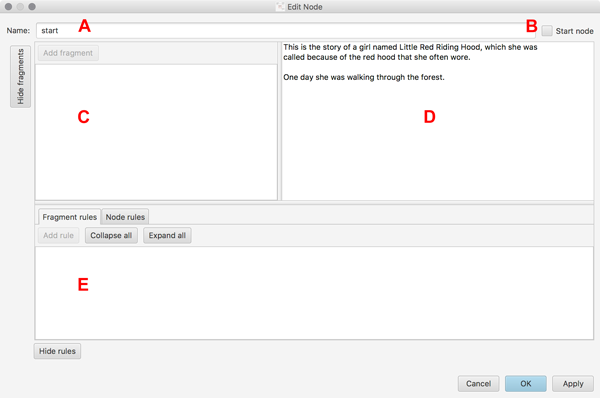
\includegraphics[width=10cm]{images/hypedyn-tutorial-1-figure-5}
  \caption{\textit{The editing view of a node.}}
  \label{fig:tut1:edit_node}
\end{figure} 

The Edit Node window lets you rename a node and enter the text for a node. It also lets you add, edit and delete fragments and rules. The Edit Node window consists of the \textit{Node name} (A), the \textit{Start node} checkbox (B), the \textit{Fragment list} (C), the \textit{Content editor} (D), and the \textit{Rules list} (E).

\item Now enter the text for the first fragment of our story in the Content editor:

\textit{This is the story of a girl named Little Red Riding Hood, which she was called because of the red hood that she often wore.}

\textit{One day she was walking through the forest.}

\item We want this node to be the start of our story, so click on the \textit{Start node} checkbox at the top right of the  to set this node as the start node. Every story must have a start node. The start node is indicated by the words ``(start node)'' shown after the node name in the Map view. % this is not yet true, need to add this
\item Once you've finished entering this text, close the Edit Node window by clicking on the ``Ok'' button. This will take you back to the Map view.
\end{enumerate}

\section{Creating links between nodes}

We will now create several other nodes to contain the rest of our hypertext story, and we'll create links between them.

\subsection{Creating the other nodes}

\begin{enumerate}
  \item Create another text node, and name it ``forest''.
  \item Enter the following text in the node:

\textit{In the forest, Red came across a young man with a nasty smile.}

\textit{``Where are you going, little girl?'' he asked.}

\textit{``I'm off to see my sick granny,'' she said.}

\textit{Well, you can probably guess what happened next.}

This node represents the main conflict of the story.

\item Create a third node, and name it ``end''.
\item Enter the following text in the node:

\textit{*** The End ***}

\textit{back to start}

This node represents the end of our story.
\end{enumerate}

You should have three nodes: ``start'', ``forest'', and ``end'', as in
Figure \ref{fig:tut1:three_nodes}.
 
\begin{figure}[ht]
  \centering
  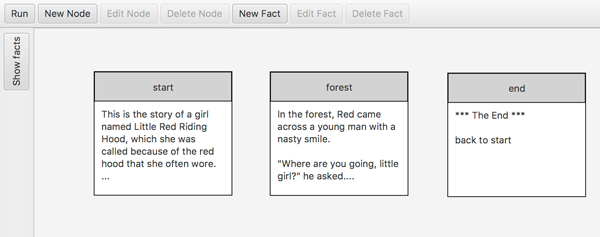
\includegraphics[width=12cm]{images/hypedyn-tutorial-1-figure-6}
  \caption{\textit{Three text nodes.}}
  \label{fig:tut1:three_nodes}
\end{figure} 

\subsection{Creating a link}

Now we want the reader to be able to move from one node to another, as they make decisions about how to read the story. To do this, we need to create \textit{links} between the nodes.

Links in HypeDyn can be attached to a specific piece of text, called a \textit{fragment}. When the reader clicks on a fragment, one or more rules are triggered. These rules are where the author can specify what will happen when the fragment is clicked. For example, in our
story, we want the user to be able to click on ``forest'' in the ``start'' node to jump to the ``forest'' node. This lets the user progress through the main story path. 

\begin{enumerate}
  \item Select the ``start'' node in the Map view, and then click on the Edit node button.
  \item Now select the word ``forest''. We'll attach our link here.
  \item Click on the \textit{Add fragment} button above the fragment list in the Editing view. A new fragment will be added to the fragment list, and it will be named ``new fragment'', as shown in Figure \ref{fig:tut1:create_link}.

\begin{figure}[ht]
  \centering
  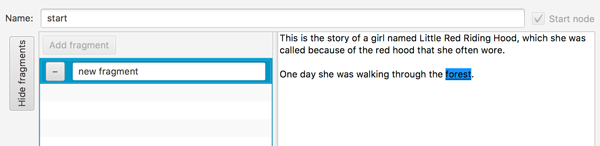
\includegraphics[width=10cm]{images/hypedyn-tutorial-1-figure-7}
  \caption{\textit{Creating a fragment.}}
  \label{fig:tut1:create_link}
\end{figure} 

\item Give the fragment a name, such as ``Next''. Notice that fragments show up as underlined text in the content editor of the Edit Node window.
\item Directly below the fragment list, you can see the \textit{fragment rules list} (see Figure \ref{fig:tut1:edit_link_1}). This is where
we can specify the rules for the fragment to create our link.

The fragment rules list consists of a list of rules, each of which will be triggered when the user clicks on the fragment. For now, we will create a single rule, which will create a link to jump the story to the ``forest'' node.

\begin{figure}[ht]
  \centering
  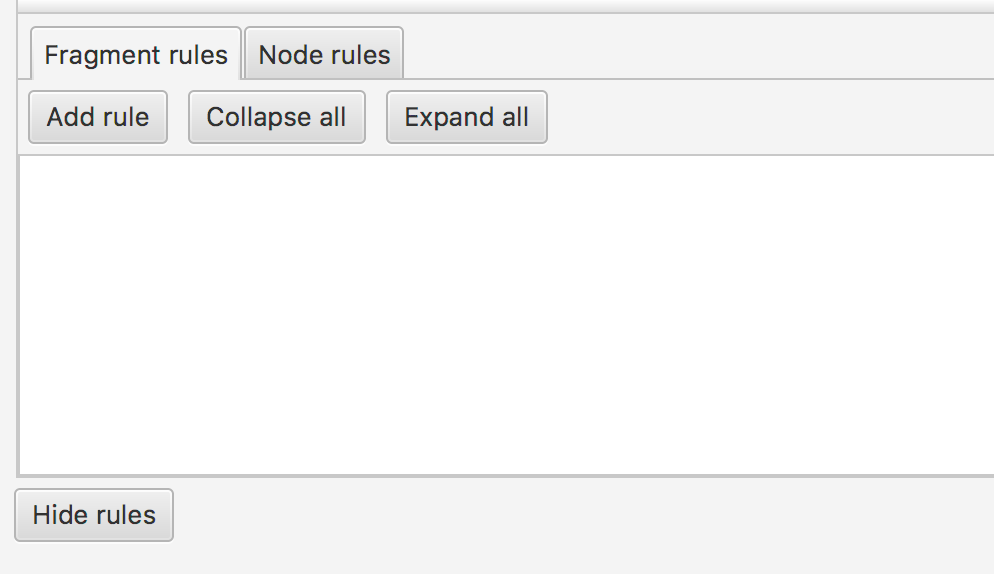
\includegraphics[width=9cm]{images/hypedyn-tutorial-1-figure-8}
  \caption{\textit{The fragment rules list.}}
  \label{fig:tut1:edit_link_1}
\end{figure} 

\item Make sure that the fragment you just created is selected in the fragment list. Now click on the \textit{Add rule} button at the top left of the fragment rules list. A rule, named ``New Rule'', will be added to the list of fragment rules (see Figure \ref{fig:tut1:new_rule}).

\begin{figure}[ht]
  \centering
  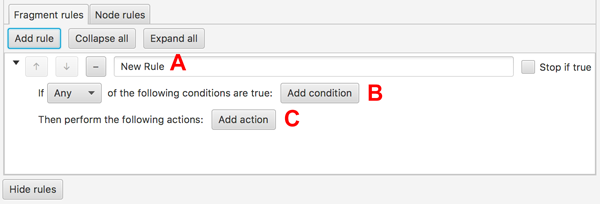
\includegraphics[width=10cm]{images/hypedyn-tutorial-1-figure-8b}
  \caption{\textit{Adding a rule to the fragment rules list.}}
  \label{fig:tut1:new_rule}
\end{figure} 

Every rule consists of three sections: the \textit{rule name} (A) which allows you to edit the name of the rule, the \textit{conditions} (B)
listing a series of conditions which specify when the rule can be triggered, and the \textit{actions} section (C) which is the set of actions that are performed when the conditions are satisfied. For now we are just going to add an action to our rule. We will return to conditions below.

\item First edit the name of the rule, changing it to ``Next''. This is the label which will be placed on the link when it is displayed in the Map view.

\item Next, create the action. Click on the \textit{Add action} button in the rule. An action will be added to the action list.

\item In the new action, select ``follow link to'' in the first pull-down menu. Then use the second pull-down menu to choose the ``forest'' node. This will create a link from the text ``forest'' in the ``start'' node to the ``forest'' text node (see Figure \ref{fig:tut1:create_action}).

\begin{figure}[ht]
  \centering
  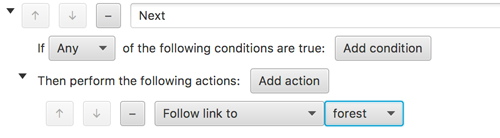
\includegraphics[width=9cm]{images/hypedyn-tutorial-1-figure-8d}
  \caption{\textit{Creating the rule to follow a link from ``start'' to
  ``forest''.}}
  \label{fig:tut1:create_action}
\end{figure} 

\item Now click OK in the Edit Node window to return to the main window.
\end{enumerate}

We have now created a link from the ``start'' node to the ``forest''. You should be able to see this link in the Map view, as shown in Figure \ref{fig:tut1:new_link_mapview}.
  
\begin{figure}[ht]
  \centering
  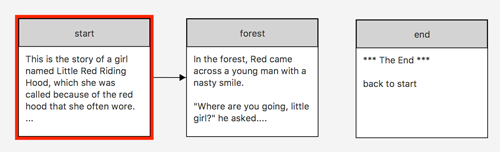
\includegraphics[width=10cm]{images/hypedyn-tutorial-1-figure-9}
  \caption{\textit{The link from the ``start'' to the ``forest''.}}
  \label{fig:tut1:new_link_mapview}
\end{figure} 

\subsection{Testing the link}

Now that we've created the link, we need to test that it works.

To test our story, we need to use the \textit{Run} button in the Toolbar in the Map view.

\begin{enumerate}
  \item Close the ``start'' node if its still open.
  \item Now click on the Run button. HypeDyn will open your story in a web browser window, showing the contents of the start node. You are now ``reading'' the story, instead of editing it, as shown in Figure \ref{fig:tut1:reading}.

\begin{figure}[ht]
  \centering
  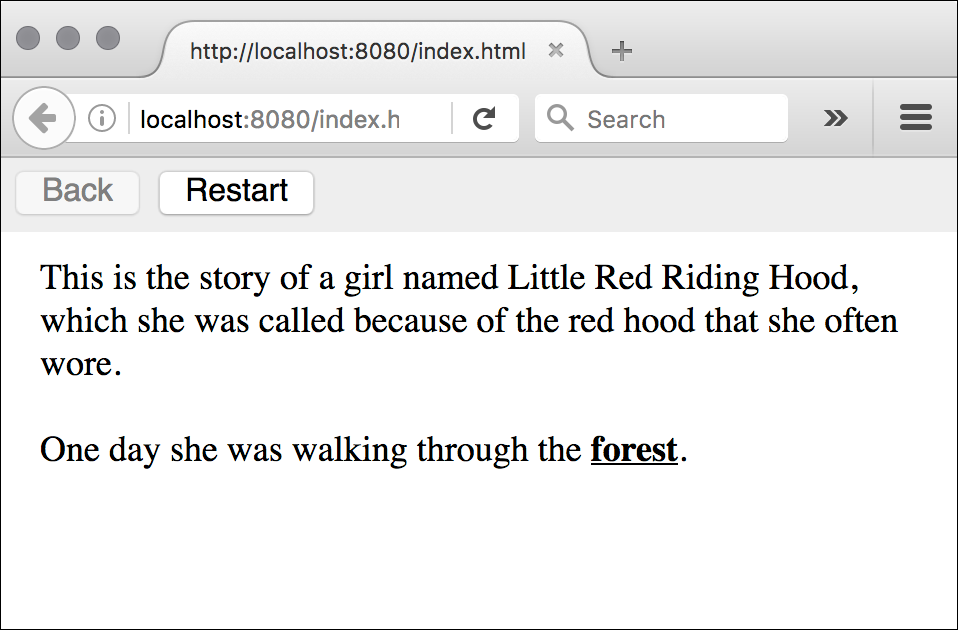
\includegraphics[width=9cm]{images/hypedyn-tutorial-1-figure-10}
  \caption{\textit{Reading a text node.}}
  \label{fig:tut1:reading}
\end{figure} 

When reading a story, you can click on links, and you'll be taken to the node that the link leads to.

\item Click on the word ``forest'' to follow the link.
\item The story will change to show the contents of the ``forest'' node.
\end{enumerate}

You can finish reading the story by closing the browser window.

\subsection{Creating more links}

Now that we have one link from the ``start'' to the ``forest'', we should link in our third node, ``end''. This will allow the user to move forward along the main story path from the ``forest'' node to the ``end'' node, the end of the story.

\begin{enumerate}
\item Open the ``forest'' node.
\item Select the word ``next''.
\item Click on the \textit{Add fragment} button.
\item Name this fragment ``to the end''.
\item Create a rule. Name the rule ``to the end''.
\item Now add a ``follow link to'' action, and select the ``end'' node in the pull-down menu.
\item Click on the Ok button, and close the Edit Node window.

You now have a link to the ``end'' text node. Test this out by running
the story. You should be able to click on the ``forest'' link to move to the ``forest'' node, and then click on ``next'' to move to the ``end'' node.
 
\begin{figure}[ht]
  \centering
  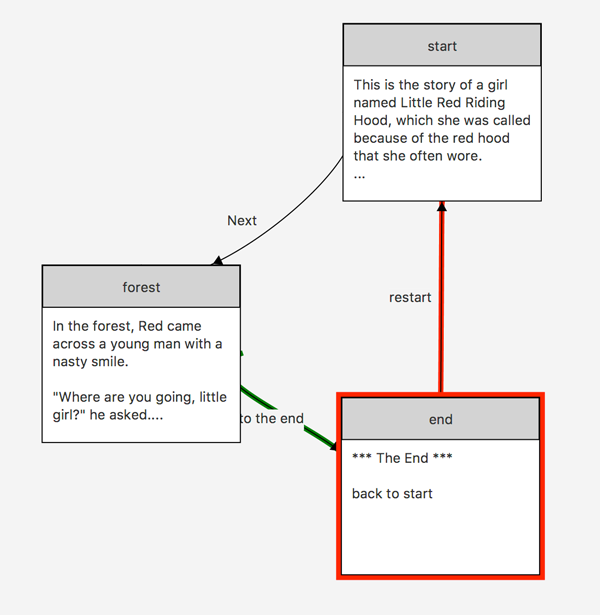
\includegraphics[width=6cm]{images/hypedyn-tutorial-1-figure-11}
  \caption{\textit{Three nodes with a loop back to the start.}}
  \label{fig:tut1:three_nodes_and_links}
\end{figure} 

Now we'll create one more link, this time from the ``end'' node back to the ``start'', so that the reader can re-read our story if they want.

\item Open the ``end'' node.
\item Select the words ``back to start''.
\item Click on the \textit{Add fragment} button.
\item Name this fragment ``restart''.
\item Create a rule, and name the rule ``restart''.
\item Now add a ``follow link to'' action, and select the ``start'' node from the pull-down menu.
\item Click on the Ok button, and close the Edit Node window.
\end{enumerate}

We now have a loop back to the start. At this point, your Map view should look as shown in Figure \ref{fig:tut1:three_nodes_and_links}.

\section{Creating rules with conditions}

The next thing we want to do is create a rule with conditions. This is a rule that can only be triggered if a certain condition, such as the user having visited a specific node, is satisfied.

We will create a node, named ``Hood details'', which can only be reached after the reader has read the entire story. This node will reveal additional information that will (hopefully) change the reader's experience of the story, as the reader will now know that there is something unusual, and perhaps slightly sinister, about Red's hood.

To do this, we will use a feature in HypeDyn called a ``condition'' to only allow the reader to see the ``Hood details'' node after they have seen the ``end'' node. This allows us, as the author of the story, to ensure that the reader has gone through the main story path at least once. We want the reader to experience the original story before seeing the new information, so that the new information can more effectively impact their previous mental model of the events of the story.

\subsection{Creating the node}

First we'll create a new node to contain the information about the hood.

\begin{enumerate}
  \item Create a new node, and name it ``Hood details''.
  \item Enter the following text in the text node:

\textit{Her hood was a magic garment, given to her by her grandmother.
It could kill anyone who tried to harm the wearer.}

\textit{But not immediately. And in a most painful manner.}

\textit{Meanwhile, in the forest\ldots}

\item Next, select the word ``forest'' in the text you just entered (in the
``Hood details'' node). Create a fragment on this word, and name the fragment
``continue''. Add a rule to the fragment, and name it ``continue''. Give the rule a ``follow link to'' action that goes to the ``forest'' node.

This link leads the reader back to the main story path, thus allowing the
reader to continue reading the story after having read the additional details in
this node.

\item Now create a link from the ``start'' node to the ``Hood details'' node.
Edit the ``start'' node and select the text ``red hood''. Create a fragment with a ``follow link to'' action that goes from this text to the ``Hood details'' node, and name the fragment and its rule ``more about the hood''.
\end{enumerate}

At this point, you should have the nodes as shown in Figure
\ref{fig:tut1:setting_up_hood_details}.
 
\begin{figure}[ht]
  \centering
  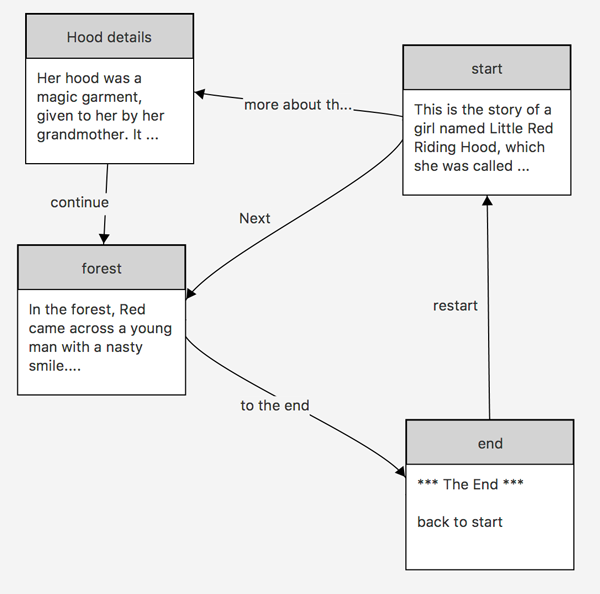
\includegraphics[width=6.5cm]{images/hypedyn-tutorial-1-figure-12}
  \caption{\textit{Setting up the ``Hood details'' node.}}
  \label{fig:tut1:setting_up_hood_details}
\end{figure} 

\subsection{Adding the condition}

Now we want to make sure that the reader can only follow the ``more about the
hood'' link if they've already read the ``end'' node. To do this, we need to
add a condition to the rule on the link between the ``start'' node and the
``Hood details'' node.

\begin{enumerate}
  \item Open the ``start'' node, and select the fragment ``more about the
  hood''. The rule for this fragment will be shown in the fragment rules list.

Every rule can contain \textit{conditions} which must be true for the rule's actions to be performed. If there are multiple conditions, then you can choose whether the actions will be performed when All or when Any of the conditions are true, by using the Any/All pull-down menu. For now, leave this pull-down menu at the default, All.

\item Click on the Add condition button. This will create a new condition that must be satisfied for the actions to be performed, as shown in Figure \ref{fig:tut1:adding_condition}.
 
\begin{figure}[ht]
  \centering
  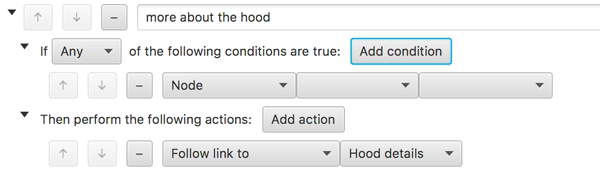
\includegraphics[width=10cm]{images/hypedyn-tutorial-1-figure-13}
  \caption{\textit{Adding a condition.}}
  \label{fig:tut1:adding_condition}
\end{figure} 

\item We want the action ``follow link to Hood details'' to only be performed if the reader has gone through the entire story at least once. This means they have to have visited the ``end'' node. Use the pull-down menus so that our condition reads ``Node end visited''. (Your condition should look like Figure \ref{fig:tut1:condition_hood_details}.) Then click Ok, and close the Edit Node window.

\begin{figure}[ht]
  \centering
  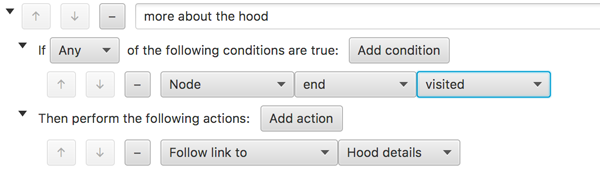
\includegraphics[width=10cm]{images/hypedyn-tutorial-1-figure-14}
  \caption{\textit{Condition for the ``more about the hood'' link.}}
  \label{fig:tut1:condition_hood_details}
\end{figure} 

\item Close the ``start'' text node.
\end{enumerate}

\subsection{Testing the rule}

Now we will test out the rule.

\begin{enumerate}
  \item In the main window, click on the Run button.
  \item In the story you should see that the text ``red hood'' is bold,
  but not underlined. This indicates a link which cannot currently be
  followed, as shown in Figure \ref{fig:tut1:start_with_condition}.
 
\begin{figure}[ht]
  \centering
  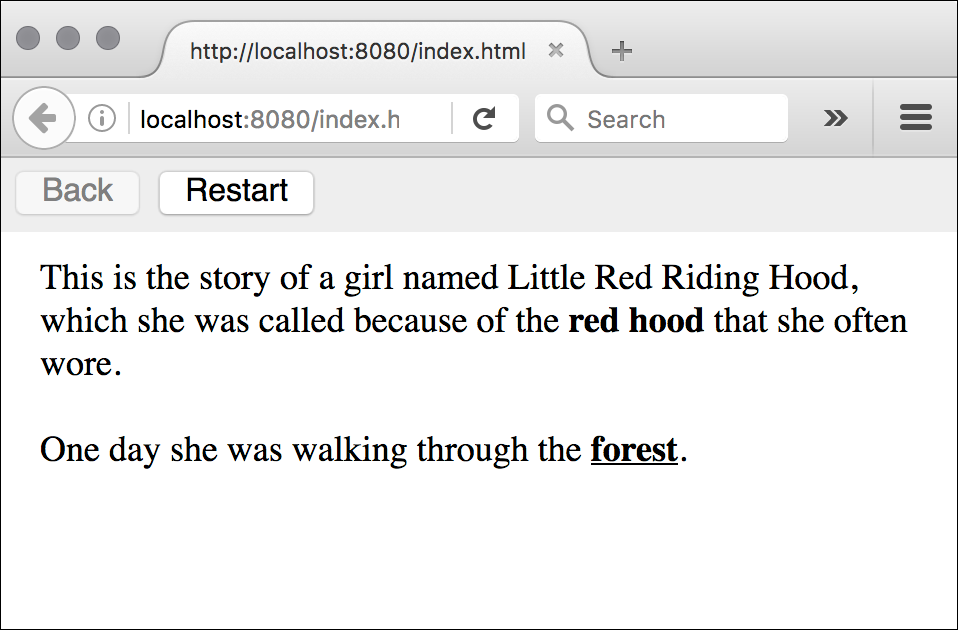
\includegraphics[width=9cm]{images/hypedyn-tutorial-1-figure-15}
  \caption{\textit{Start node with a link that cannot be followed.}}
  \label{fig:tut1:start_with_condition}
\end{figure} 

\item Now read through the story once, by clicking on ``forest'' in the
``start'' node, and then ``next'' in the ``forest'' node.
\item Finally, read back to the start by clicking on the ``back to start'' link in the ``end'' node.
\item This time, you should see that the ``red hood'' text is a normal,
followable link. Click on the link to go to the ``Hood details'' node.

\item If you want to read the story again as if you've never read it, you need to clear the story's history of which nodes have been visited.

In the browser, click on the \textit{Restart} button. The story will go to the node which we set as the start node, ``start'', and will clear its history.

\item You should now see that the ``red hood'' text is once again an
unfollowable link.
\end{enumerate}

We have now created a simple story, with links and conditions.

\section{Reading the story}

Once you have created and saved your story, you can export your story so that it can be read by other people. Choose \textit{File->Export\ldots} and specify the name of the folder where you want to export your story. HypeDyn will create a folder with that name, and save your story there as a web page. The folder contains a number of supporting files, plus an ``index.html'' file. Keep all these files together.

To read your exported story, open the ``index.html'' file in a web browser. This is exactly the same as running the story from within HypeDyn.

\section{Conclusion}

In this tutorial, we have created a simple hypertext fiction. Our story has a main path, which tells a simplified version of the traditional folk tale ``Little Red Riding Hood''. Our story also has an alternative side path, which gives the reader more information about Red's hood. This alternative side path can only be read once the reader has visited the ``end'' node at the end of the main story path. Although this is a simple story, it demonstrates all the capabilities of HypeDyn 2, capabilities that are sufficient to create a more complex hypertext fiction.

Please see tutorial 2 for more advanced features: fragments with multiple rules, conditional text, and anywhere nodes.

\end{document}
